% Proseminar
% Sebastian Honegger
% FS15

\documentclass[9pt]{beamer}
\usetheme{Boadilla}  
\usepackage{wrapfig}				% Text umgibt Grafik


\title{Project Sihlstrasse}
%\subtitle{}
\institute[ETH Zurich] {Modelling and Simulating Social Systems\\ETH Zurich}

\author[Filip Meier and Sebastian Honegger]{Filip Meier and Sebastian Honegger}
\date{October 19, 2015}



\begin{document}

\begin{frame}
\frametitle{Traffic simulation Sihlstrasse}

\begin{figure}[H]
\begin{minipage}[t]{.5\textwidth}
\begin{itemize}
\item City of Zurich want to change one specific part of the sihlstrasse in a pedestrian area
\item There will be two track less: 
\begin{itemize}
\item now: two tracks direction west (Uraniastrasse), two track direction east (Sihlstrasse)
\item after: two tracks direction west (Uraniastrasse), one track direction east (Uraniastrasse)
\end{itemize}
\end{itemize}
Research Questions
\begin{itemize}
\item[1.] Are the streets  still large enough for the traffic peaks
\item[2.] What is the impact on the neighbourhood streets?
\end{itemize}

\end{minipage}\hfill
\begin{minipage}[t]{.4\textwidth}
	\centering
	\vspace{0pt}
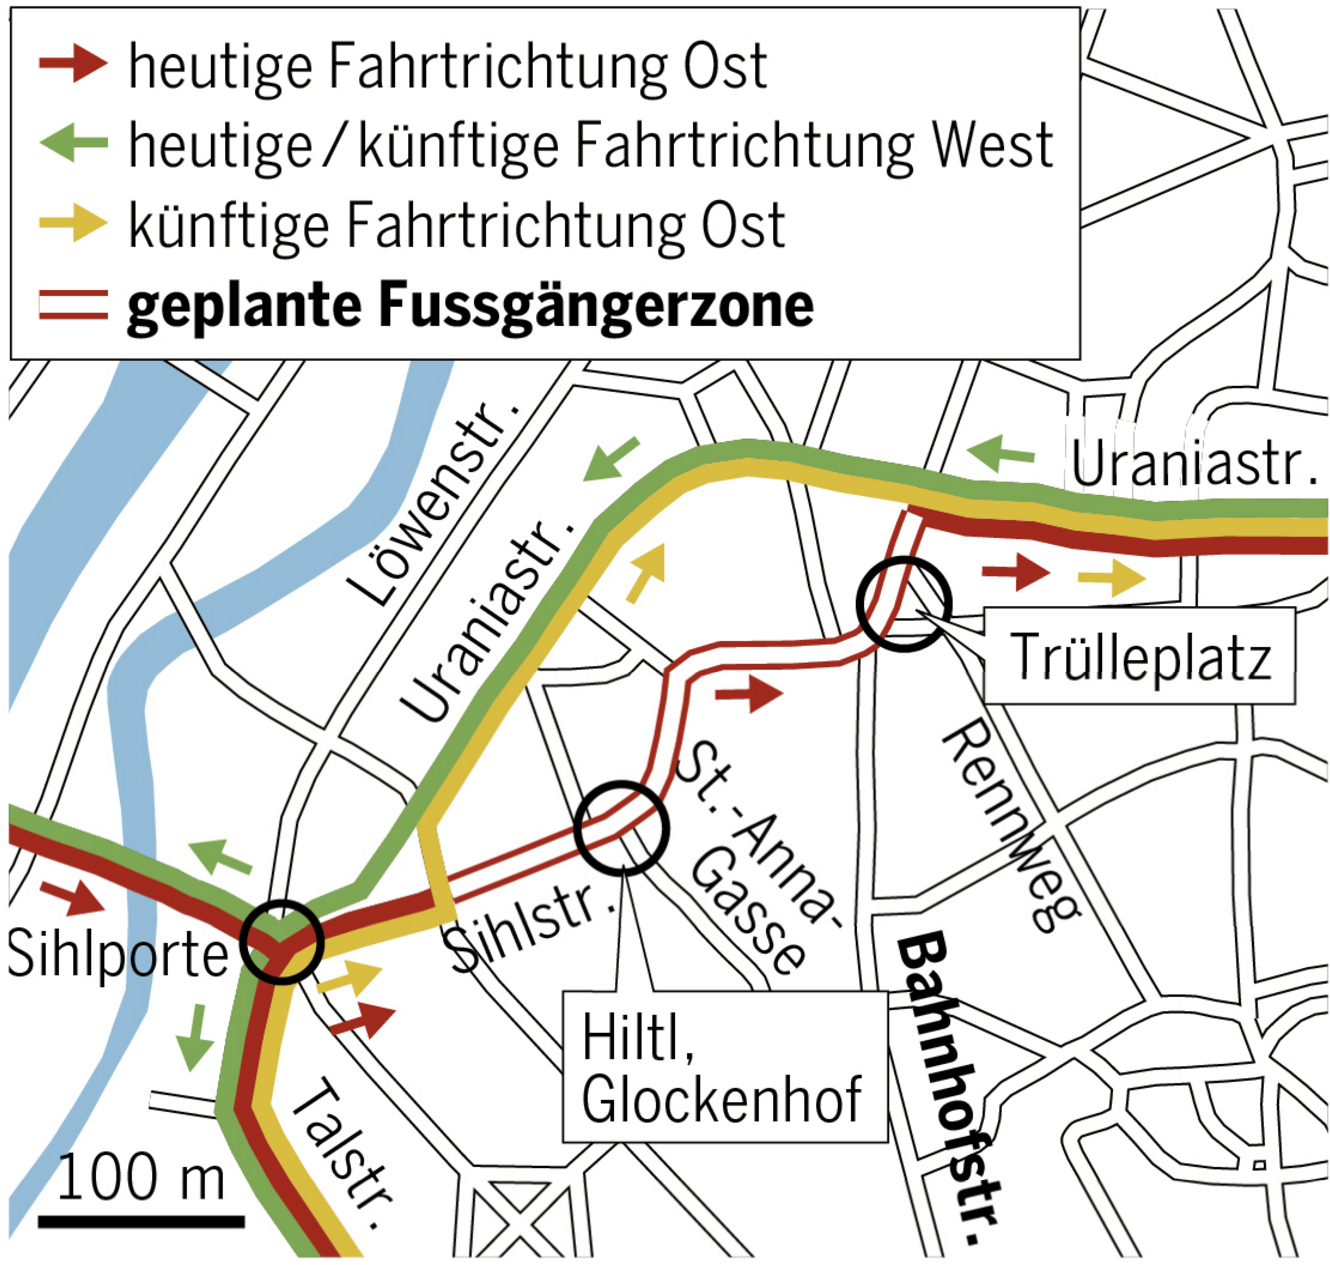
\includegraphics[width=\textwidth]{Plan_Sihlstrasse.png}
\end{minipage}\hfill
\end{figure}
Methods (examples)
\begin{itemize}
\item simulate the traffic for this area with the four steps of the classical urban transportaion planning system.
\item streets and traffic simulated by a grid 
\end{itemize}
\end{frame}



\end{document}





